\documentclass[12pt,letterpaper]{standalone}
\usepackage{tikz}
\usetikzlibrary{shapes.geometric, arrows}

\tikzstyle{startstop} = [rectangle, rounded corners, minimum width=3cm, minimum height=1cm,text centered, draw=black, fill=red!30]

\tikzstyle{io} = [trapezium, trapezium left angle=70, trapezium right angle=110, minimum width=3cm, minimum height=1cm, text centered, draw=black, fill=blue!30]

\tikzstyle{process} = [rectangle, minimum width=3cm, minimum height=1cm, text centered, draw=black, fill=orange!30]

\tikzstyle{decision} = [diamond, minimum width=3cm, minimum height=1cm, text centered, draw=black, fill=green!20, text width=4cm]

\tikzstyle{arrow} = [thick,->,>=stealth]

\begin{document}
	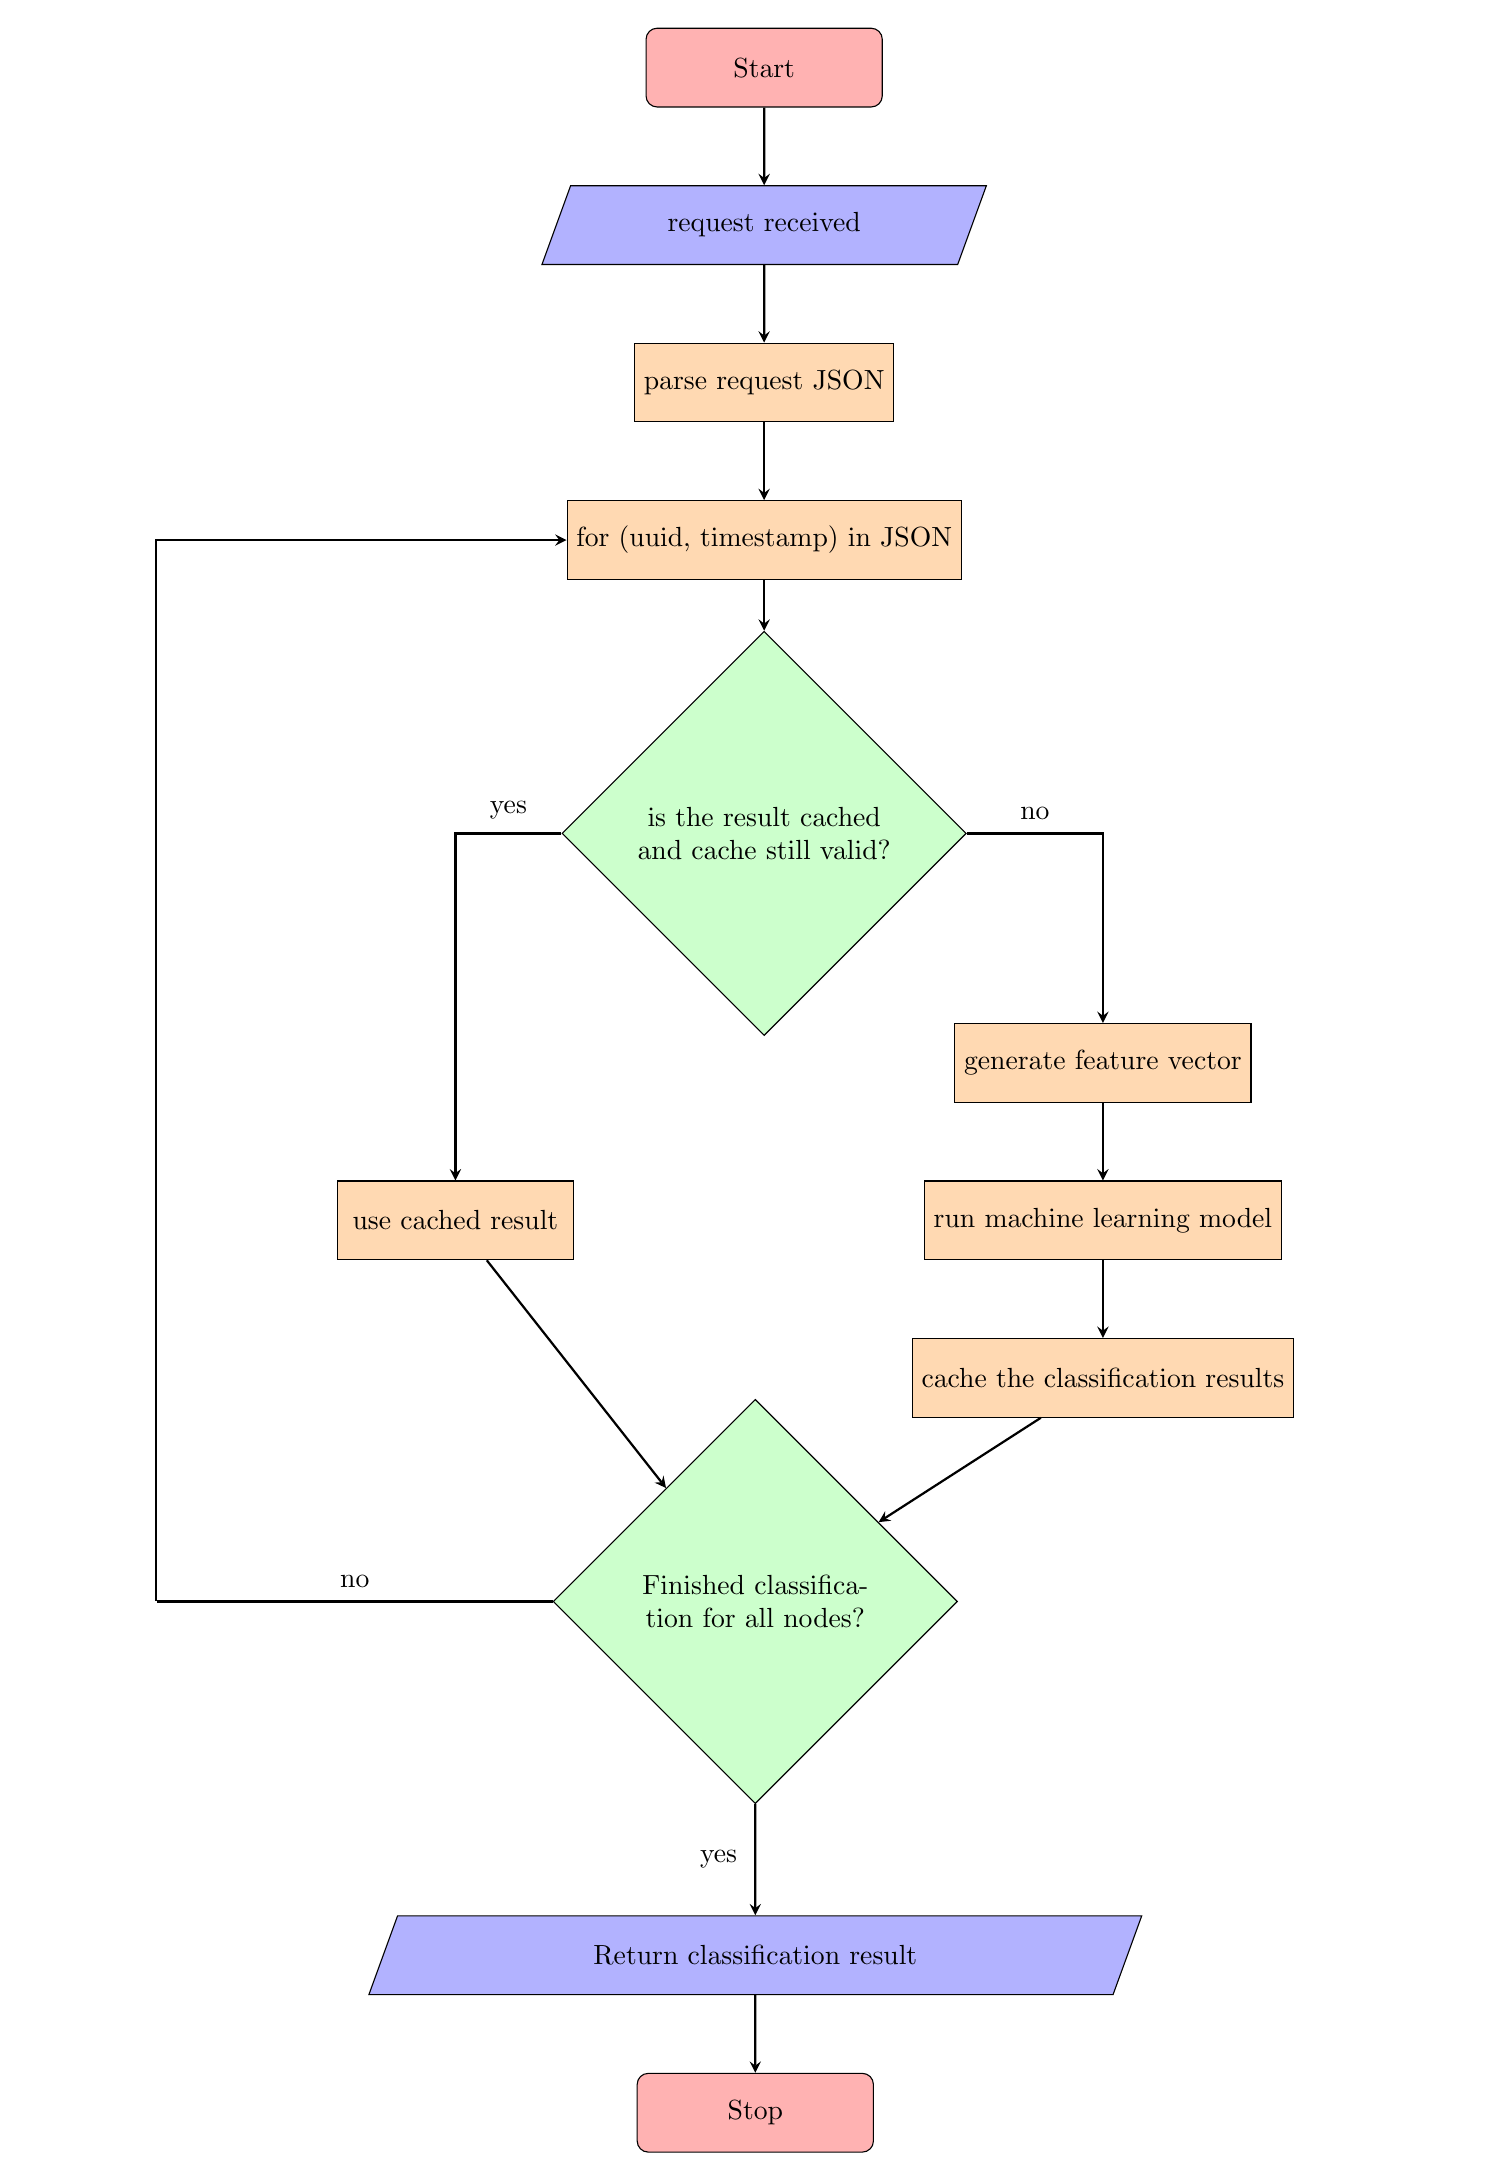
\begin{tikzpicture}[node distance=2cm]
	
		\node (start) [startstop] {Start};
		
		\node (request) [io, below of=start] {request received};
		
		\node (parse) [process, below of=request] {parse request JSON};
		\node (for-entry) [process, below of=parse] {for (uuid, timestamp) in JSON};
		\node (is-cached) [decision, below of=for-entry, above=-4.3cm] {is the result cached and cache still valid?};
		\node (use-cached) [process, below left of=is-cached, above=-3.5cm, left=1cm] {use cached result};
		\node (generate-features) [process, below right of=is-cached, above=-1.5cm, right=1cm] {generate feature vector};
		\node (run-model) [process, below of=generate-features] {run machine learning model};
		\node (cache-result) [process, below of=run-model] {cache the classification results};
		\node (ran-all) [decision, below left of=cache-result, left=3.0cm, above=-4cm] {Finished classification for all nodes?};
		\node (return) [io, below of=ran-all, above=-3cm] {Return classification result};
		\node (stop) [startstop, below of=return] {Stop};
		
		\node[scale=0.05] (dummy) [left of=ran-all, left=150cm] {};
		\node (d) [left of=ran-all, left=7cm] {}; 
		\node (d) [right of=ran-all, right=7cm] {}; 
		
		\draw[arrow] (start) -- (request);
		\draw[arrow] (request) -- (parse);
		\draw[arrow] (parse) -- (for-entry);
		\draw[arrow] (for-entry) -- (is-cached);
		\draw[arrow] (is-cached) -| (generate-features) node[near start, above=0.05cm] {no};
		\draw[arrow] (is-cached) -| (use-cached) node[near start, above=0.05cm] {yes};
		\draw[arrow] (generate-features) -- (run-model);
		\draw[arrow] (run-model) -- (cache-result);
		\draw[arrow] (cache-result) -- (ran-all);
		\draw[arrow] (use-cached) -- (ran-all);
		\draw[thick] (ran-all) -- (dummy) node[midway, above=0.05cm] {no};
		\draw[arrow] (dummy) |- (for-entry);
		\draw[arrow] (ran-all) -- (return) node[midway, left=0.1cm] {yes};
		\draw[arrow] (return) -- (stop); 
	\end{tikzpicture}
\end{document}